\section{Proposed Architecture} \label{arch}

\subsection{Overview}

TorCoin runs as a standalone service, and requires no modification of the core
Tor codebase. The system can be broken into four components, which share code
across clients and relays, but behave differently depending on role. Figure 3.1
shows a basic overview of their architecture.

\begin{figure}
  \centering
    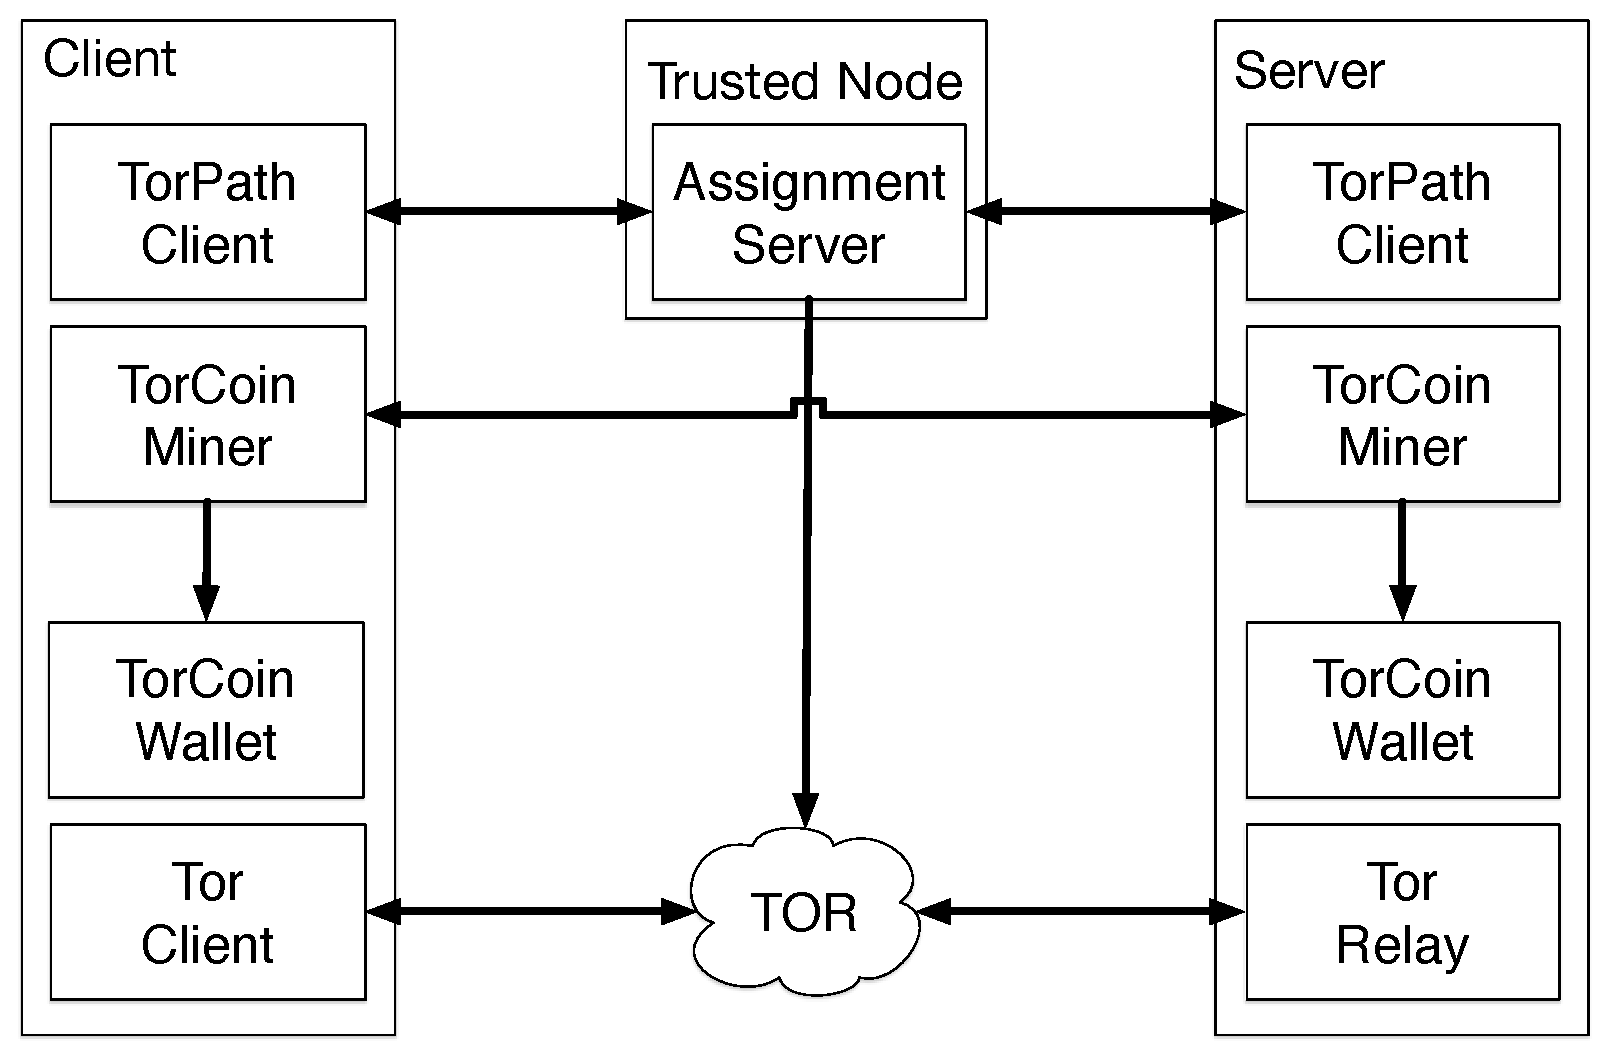
\includegraphics[scale=0.3]{architecture.pdf}
  \caption{High level TorCoin system architecture. Note that a ``trusted node''
  replaces a directory server, and actually improves on its anonymity properties.}
\end{figure}

We will briefly describe the role of each component in the system. Then, the
next two sections will describe the detailed implementations of the TorPath
protocol and TorCoin algorithm.

\subsection{TorPath Components} TorPath is an anonymous cooperative routing
scheme that randomly assigns circuits to Tor clients using decentralized,
cryptographically verifiable methods. It requires a group of assignment servers,
which are ``collectively trusted'' in the same way that Tor directory servers are, and a TorPath
client to communicate with them. 

\subsubsection{Assignment Server} A small set of trusted nodes run the
Assignment Servers, which perform similar roles to the current Tor directory 
servers. Groups of assignment servers use the distributed TorPath protocol to 
keep track of available relays and assign circuits to clients.

\subsubsection{TorPath Software} Clients and relays install the TorPath Software to
communicate with Assignment Servers, using the TorPath protocol to retrieve
circuits (clients). 
% To avoid modifying Tor client code, TorPath can use a local 
% DNS proxy to redirect requests to directory servers to the new assignment servers.

\subsection{TorCoin Components} These components implement the TorCoin algorithm
in order to reward nodes for transferring bandwidth. We describe the TorCoin 
algorithm in depth in its own section, so here we only briefly outline the 
components required to implement it.

\subsubsection{TorCoin Miner} To mine TorCoins, clients and relays that are part
of a circuit communicate via the TorCoin miner, which implements the TorCoin
algorithm. The TorCoin miner measures Tor bandwidth by monitoring the the 
throughput of the local Tor TLS tunnel, allowing us to avoid modifying internal 
Tor code.

\subsubsection{TorCoin Wallet} Since TorCoin is based on the BitCoin protocol,
it uses a cryptographic wallet for storage of coins and transactions. When the
miner discovers a new TorCoin, it adds it to the blockchain with all the
information necessary fro anyone to verify it.
